\section{Introducción}

\subsection{Área temática}
\begin{frame}{Área temática}
	Este trabajo se basa en 5 pilares teóricos:
	\medskip
	\begin{itemize}[<*>]
		\item Sistemas de Recomendación.
		\item Sitios de Community Question Answering (CQA).
		\item Medidas de similaridad.
		\item Ensamble de Clustering.
		\item Big Data.
	\end{itemize}
\end{frame}

\begin{frame}{Área temática II}
	\textbf{Area temática}
	\medskip
	\begin{itemize}
		\item Miles de nuevas preguntas son formuladas diariamente en sitios de CQA como Yahoo! Answers, Stackexchange, Stackoverflow, o Quora.
		\item Muchas de las preguntas no están respondidas correctamente o no tienen respuestas.
		\item Es de interés buscar si esa misma pregunta ha sido formulada por otro usuario previamente, y que tenga la respuesta buscada.
		\item Preguntas que poseen la misma respuestas estan formuladas de forma difente en el sentido léxico.
		\item Es necesaria una medida de similaridad que tenga en cuenta caracteristicas léxicas y semánticas.
		\item La tarea de recomendar preguntas similares en sitios de CQA puede ser llevada a cabo por un RS.
		\item Se diseñó e implementó una arquitectura Big Data para crear una medida de similaridad que alimente a un RS para sitios de CQA.	\end{itemize}
\end{frame}


\subsection{Tema específico}
\begin{frame}[allowframebreaks]{Tema específico}
	Pipeline para un RS basado en contenido de CQA y en una nueva medida de similaridad.
	\medskip
	\begin{figure}
		\centering
		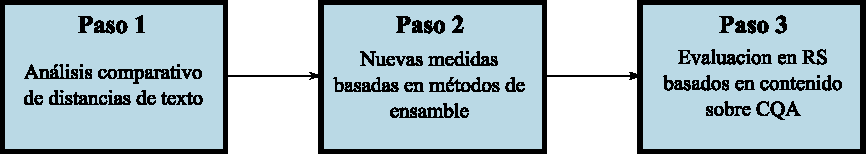
\includegraphics[width=0.7\linewidth]{../5_introduccion/imagenes/pipeline}
		\label{fig:pipeline}

		\framebreak

		Considerando el conjunto completo de datos Quora (\(404301\) pares de preguntas, es decir, \(808602\) preguntas totales), deberiamos realizar:

		\bigskip $\frac{n(n+1)}{2} = 326919001503$ calculos de distancias, donde $n = 808602$
	\end{figure}
\end{frame}

\subsection{Objetivo general}
\begin{frame}{Objetivo general}
	\begin{tcolorbox}[colback=blue!5,colframe=blue!40!black,title=Objetivo general]
		Construir una \textbf{arquitectura Big Data} que incluye la posibilidad de ser aplicada a grandes conjuntos de datos de \textbf{preguntas en el ámbito de CQA} y, a partir de esta arquitectura, implementar y evaluar nuevas \textbf{medidas de similaridad} entre textos que puedan ser utilizadas en \textbf{Sistemas de Recomendación}.
	\end{tcolorbox}
\end{frame}

\subsection{Objetivos específicos}
\begin{frame}{Objetivos específicos}
	\begin{tcolorbox}[colback=blue!5,colframe=blue!40!black,title=Objetivos específicos]
		\begin{scriptsize}
			\begin{itemize} [<+>]
				\item Diseñar y desarrollar una \textbf{arquitectura Big Data} para cálculo de similaridad en grandes matrices, que requerirá nuevas estrategias para recolectar, procesar y manejar grandes volúmenes de datos.
				\item Identificar \textbf{medidas de similaridad de texto} existentes y un método efectivo de aplicación de las mismas en grandes volúmenes de datos.
				\item Evaluar el comportamiento de \textbf{medidas de similaridad de texto} del estado del arte respecto al manejo del \textbf{volumen, variedad, velocidad y veracidad} inherentes a grandes volúmenes de datos, en particular en el \textbf{ámbito de CQA}.
				\item \textbf{Proponer una nueva medida} que permita integrar las medidas de similaridad del estado del arte mediante una arquitectura de software basada en Big Data y que sea extensible a otras medidas existentes en el estado del arte.
				\item \textbf{Brindar conclusiones, pautas y recomendaciones} para trabajar con medidas de comparación de textos en grandes volúmenes de datos en sitios de CQA utilizando arquitecturas basadas en Big Data.
			\end{itemize}
		\end{scriptsize}
	\end{tcolorbox}
\end{frame}